\section{Regression accuracy}
This section includes an examination of the accuracy of the regressors. This will be examined through superimposition of the regressor outputs on the estimated data, and through RMSE plots. To evaluate how the regressors perform with new data, a test with new data of 50 $\%$ of the MVC of all movements in all limb positions will be fed the regressor and the above examination of accuracy will be performed. 

The plot in \figref{fig:SuperPositionTestDataLogVar} depicts the actual data superimposed on the estimated data from the regressors trained with the logarithmic variance features. 

\begin{figure}[H]
	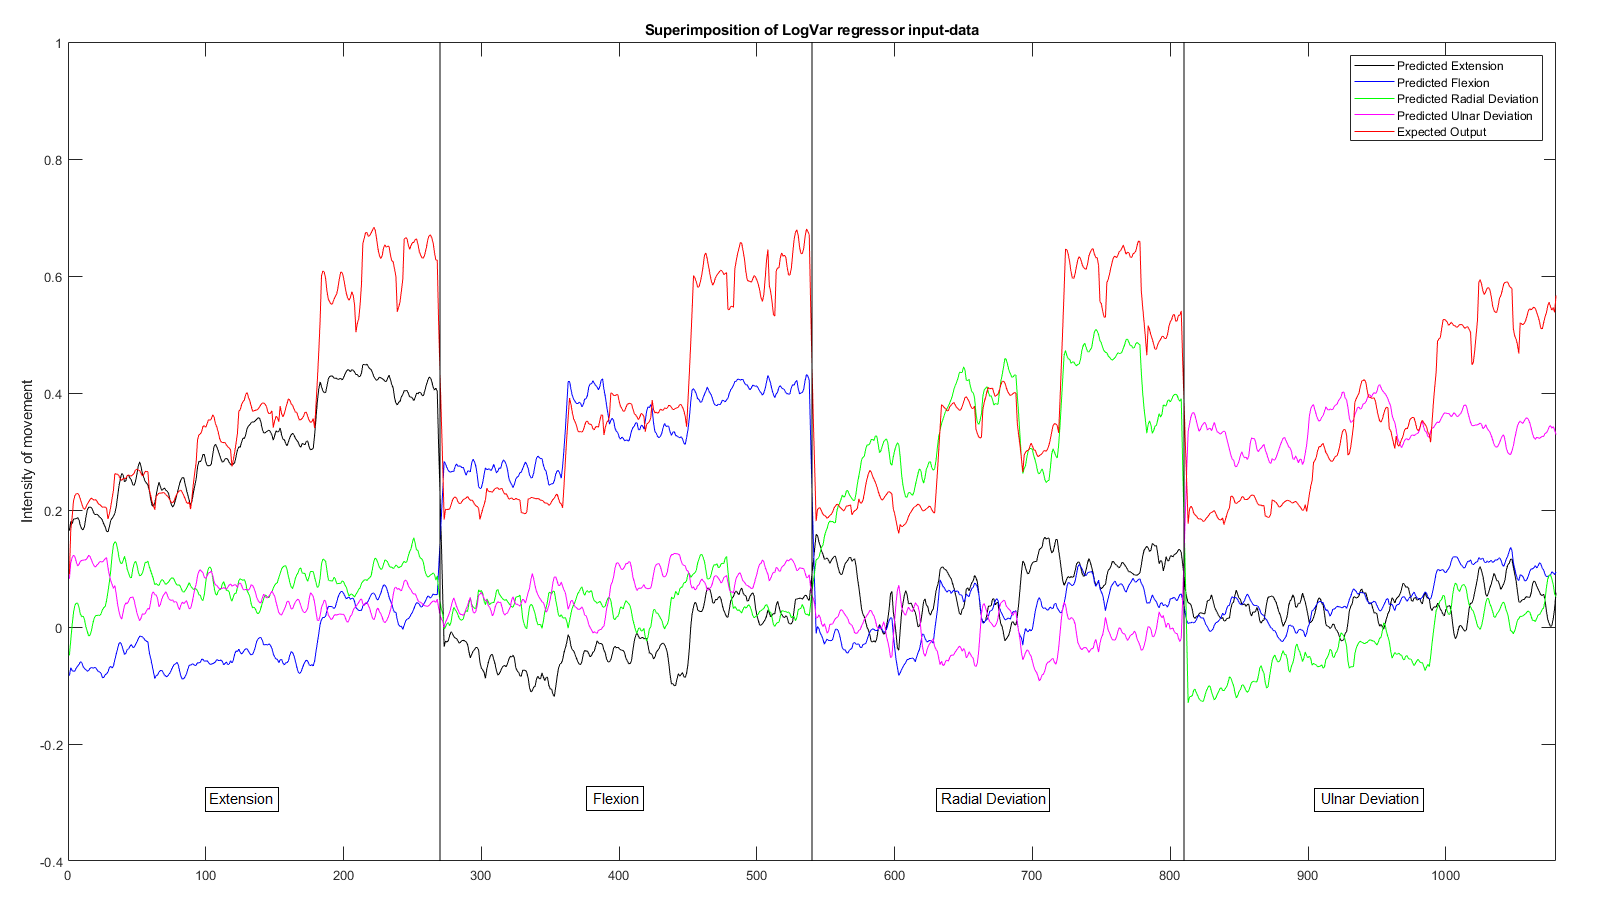
\includegraphics[width=0.7\textwidth]{figures/results/SuperPositionTestDataLogVar}  %<--but is not needed.
	\caption{Plot of the actual data, red plot, superimposed on the output of the regressors trained with the logarithmic variance features. The plot is divided into four segments, where each segment shows a different movement performed. Each segment has the same sample size.}
	\label{fig:SuperPositionTestDataLogVar}  %<--give the figure a label, so you can reference!
\end{figure}

The plot in \figref{fig:SuperPositionTestDataMAV} depicts the actual data superimposed on the estimated data from the regressors trained with the MAV features. 

\begin{figure}[H]
	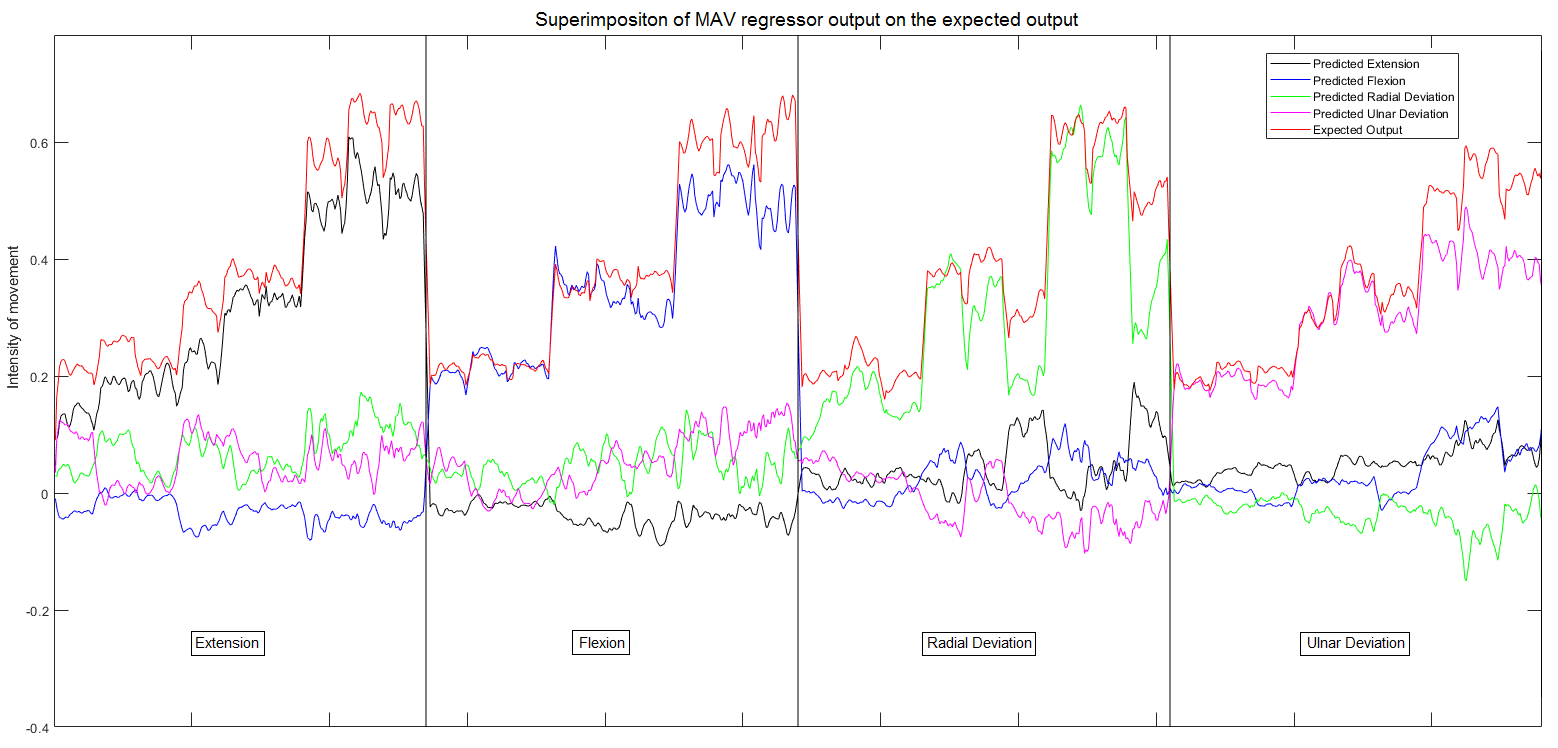
\includegraphics[width=0.7\textwidth]{figures/results/SuperPositionTestDataMAV}  %<--but is not needed.
	\caption{Plot of the actual data, red plot, superimposed on the output of the regressors trained with the MAV features. The plot is divided into four segments, where each segment shows a different movement performed. Each segment has the same sample size.}
	\label{fig:SuperPositionTestDataMAV}  %<--give the figure a label, so you can reference!
\end{figure}


A qualitative examination of the plots shows that each regressor reacts on the movement it is fitted for, and remains inactive when another movement is performed. This accounts for both features. Both regressors has a lower accuracy in the high intensities, especially for the regressors trained with logarithmic variance features. 
%regression on MAV features yields a more accurate output than regression on the logarithmic variance feature, whereas both estimates yield inaccurate fitting in the high intensities. However, both estimates yield inaccurate fitting in the high intensities compared to the lower intensities, especially in the ulnar deviation movement.
  


Calculating the RMSE of the regressors for the MAV and logarithmic variance features of the training data across all subjects, yields the results depicted in \figref{fig:gimmeThemRMSEBars}. 

\begin{figure}[H]
	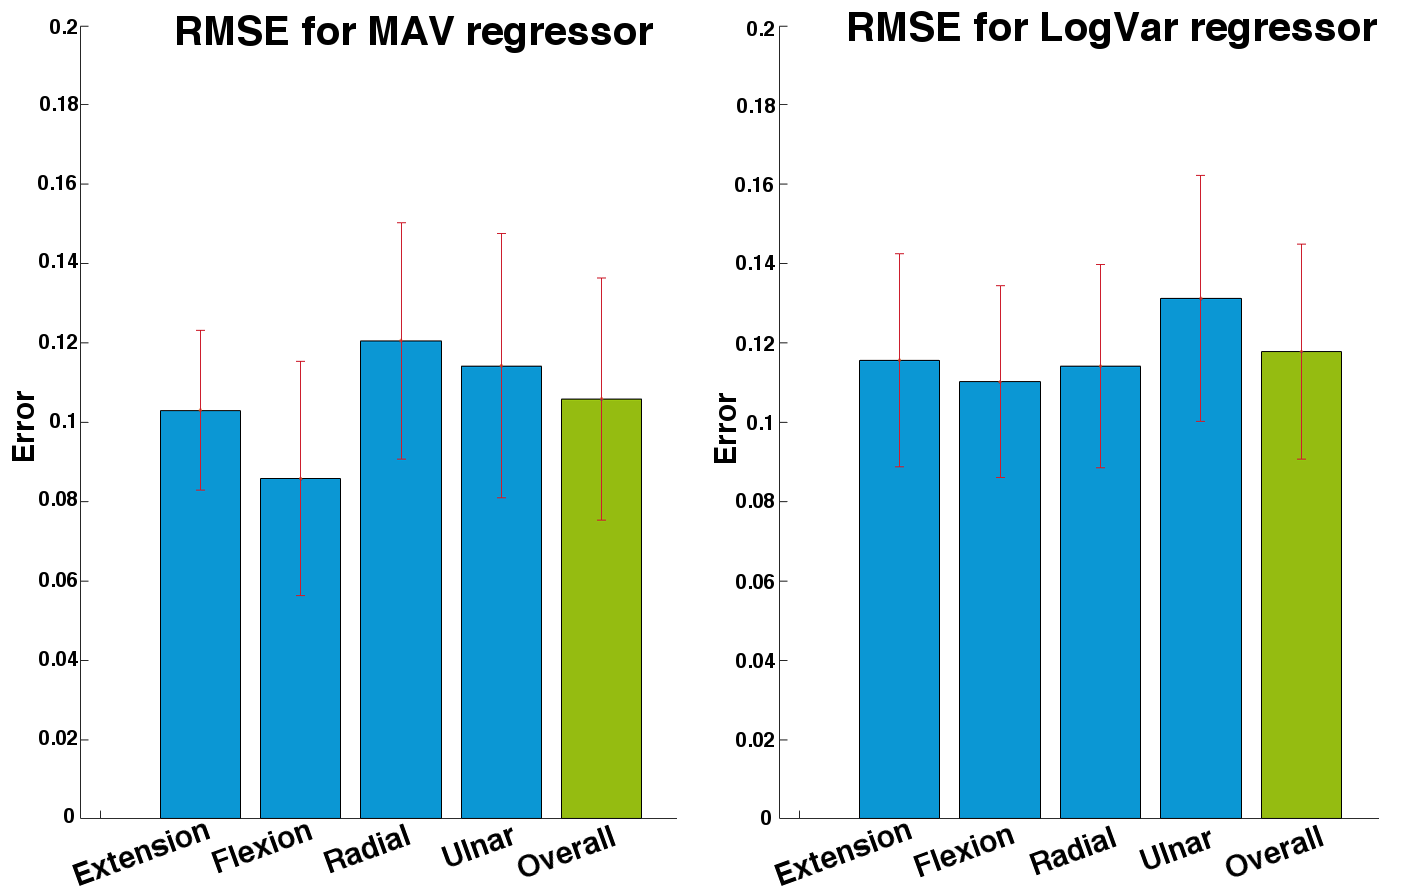
\includegraphics[width=.7\textwidth]{figures/results/gimmeThemRMSEBars}  %<--but is not needed.
	\caption{Bar plot of the error of MAV and the logarithmic variance features for the four hand gestures. The bar chart illustrates the mean error and the error bar illustrates the standard deviation}
	\label{fig:gimmeThemRMSEBars}  %<--give the figure a label, so you can reference!
\end{figure}

The overall mean of the RMSE of MAV is 0.0943 with a standard deviation of $\pm 0.0290$, where the highest mean of a regressor is 0.1088 and the highest standard deviation is $\pm 0.0366$. The overall mean of the RMSE of the logarithmic variance is 0.1107 with a standard deviation of $\pm 0.0298$, where the highest mean of a regressor is 0.1216 and the highest standard deviation is $\pm 0.0402$. MAV then yields a lower mean RMSE and a lower standard deviation than the logarithmic variance - both with the overall RMSE and for the movement with the highest RMSE. 

%%% testing data plot
\subsection{Accuracy of regressors with test data}
This section contains the superimposition of the expected output of the regressors on the output of the regressors fed with test data. The plot in \figref{fig:SuperPoisonLogVarNewData} depicts the superimposition the logarithmic variace trained regressors fed with the test data.

\begin{figure}[H]
	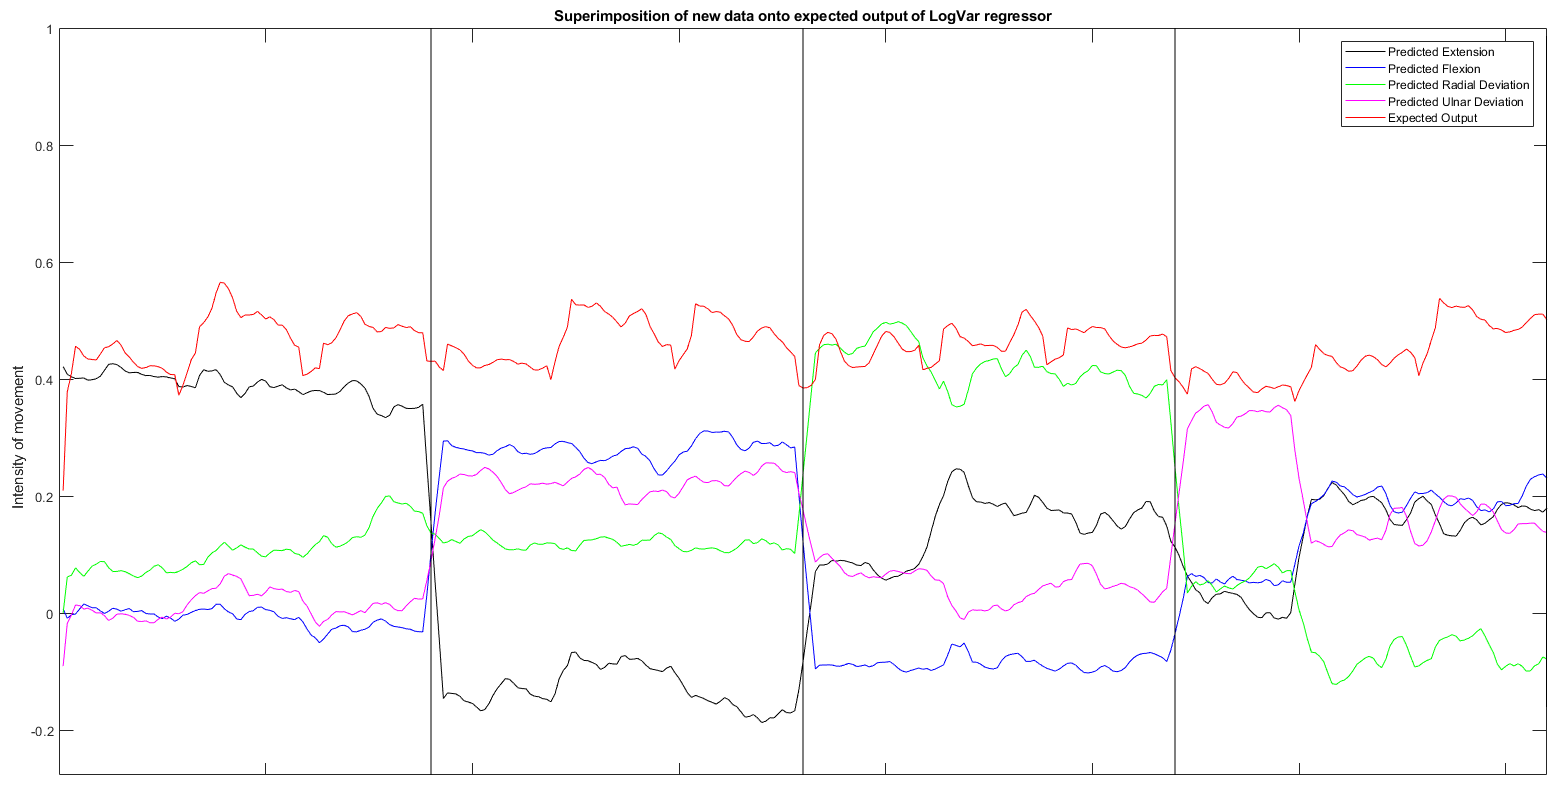
\includegraphics[width=0.7\textwidth]{figures/results/SuperPoisonLogVarNewData}  %<--but is not needed.
	\caption{}
	\label{fig:SuperPoisonLogVarNewData}  %<--give the figure a label, so you can reference!
\end{figure}

It is seen that regressors trained for different mobv reacts on the same movement, especially for the flexion and ulnar deviation movement. However, the 

\begin{figure}[H]
	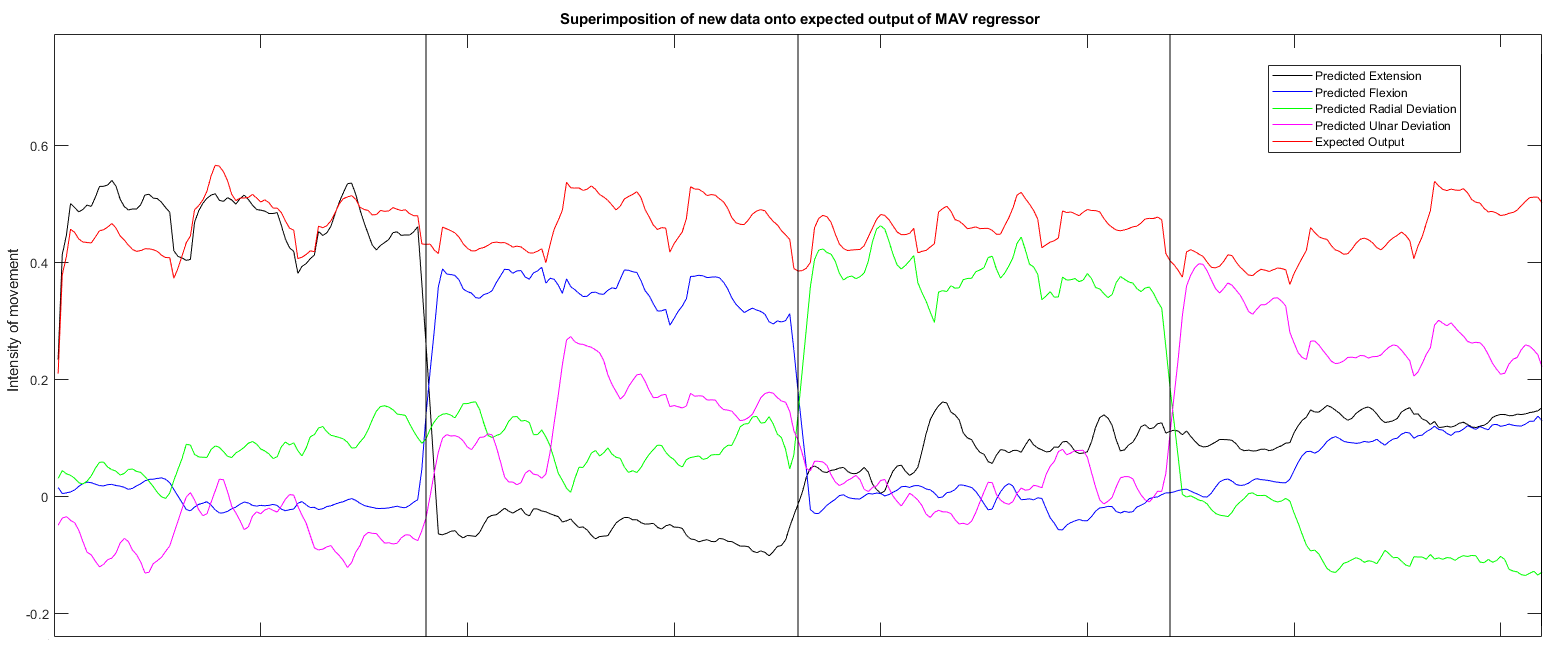
\includegraphics[width=0.7\textwidth]{figures/results/SuperPoisonMavNewData}  %<--but is not needed.
	\caption{}
	\label{fig:SuperPoisonMavNewData}  %<--give the figure a label, so you can reference!
\end{figure}


\begin{figure}[H]
	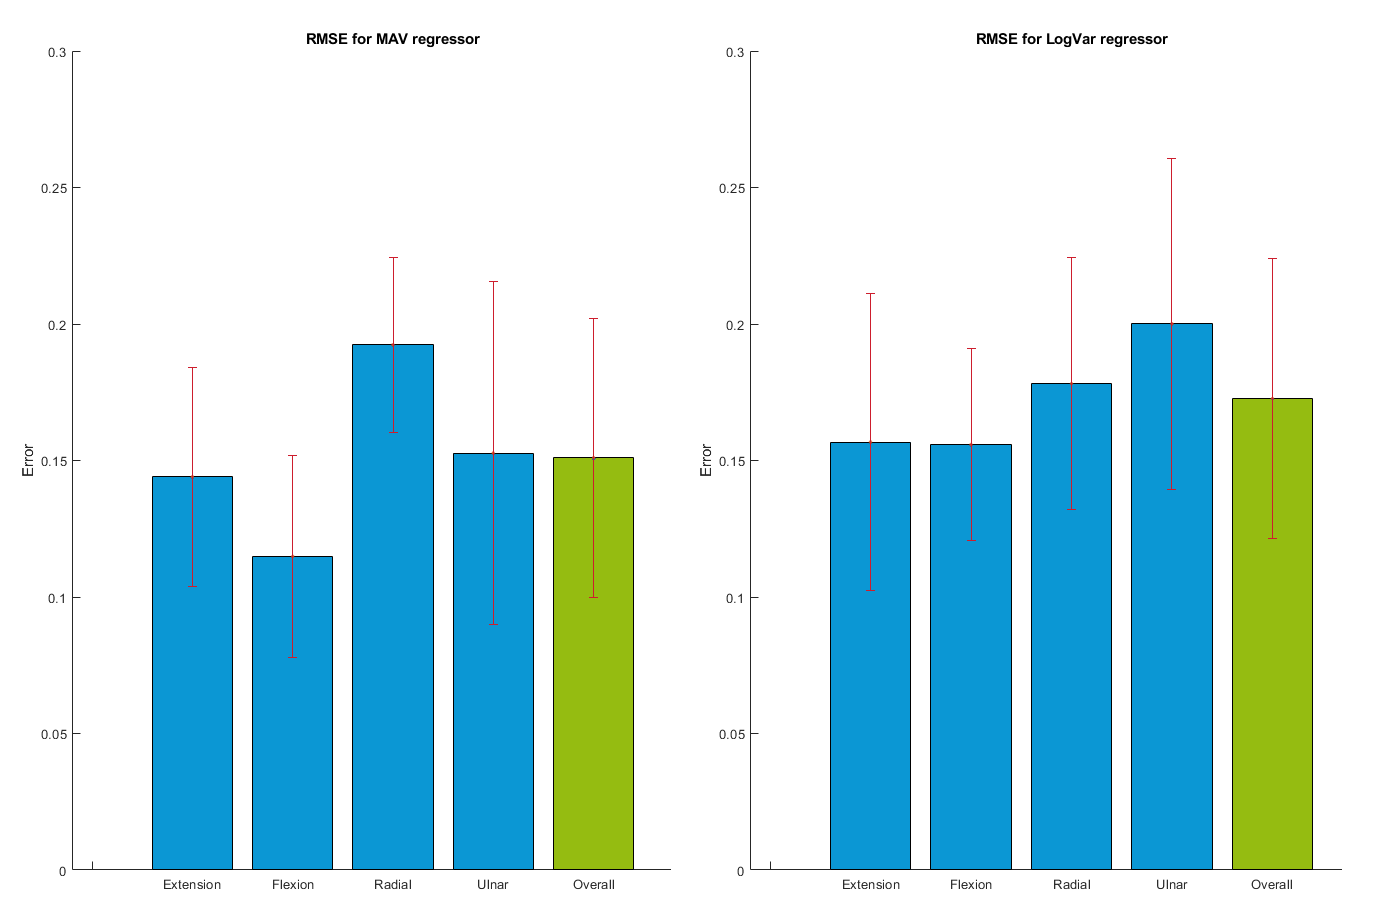
\includegraphics[width=0.7\textwidth]{figures/results/RMSEBarPlotNewData}  %<--but is not needed.
	\caption{}
	\label{fig:RMSEBarPlotNewData}  %<--give the figure a label, so you can reference!
\end{figure}
